\documentclass{article}
\usepackage[utf8]{inputenc}
\usepackage[english]{babel}
\usepackage [autostyle, english = american]{csquotes}
\MakeOuterQuote{"}
\usepackage{graphicx}
\usepackage{enumerate}
\usepackage{float}
\graphicspath{ {} }
\usepackage{mathtools}
\usepackage{amsmath, amsthm, amssymb, amsfonts}
\usepackage{caption}
\usepackage{bm}
\usepackage{fancyhdr}
\pagestyle{fancy}
\fancyhf{}
\rhead{Ty Darnell}
\lhead{Homework 10}

% For derivatives
\newcommand{\deriv}[1]{\frac{\mathrm{d}}{\mathrm{d}x} (#1)}

% For partial derivatives
\newcommand{\pderiv}[2]{\frac{\partial #1}{\partial #2}}

% Integral dx
\newcommand{\dx}{\mathrm{d}x}
\newcommand{\cd}{\overset{d}{\to}}
\newcommand{\cp}{\overset{p}{\to}}
\newcommand{\B}{\beta}
\newcommand{\e}{\epsilon}
\newcommand{\limn}{\lim_{n\to \infty}}
\newcommand{\lm}{\lambda}
\newcommand{\sg}{\sigma}
\newcommand{\hb}{\hat{\beta}}
\newcommand{\sumn}{\sum_{i=1}^{n}}
\newcommand{\hth}{\hat{\theta}}
\newcommand{\lra}{\Leftrightarrow}
\newcommand{\prodn}{\prod_{i=1}^{n}}
\newcommand{\dll}[1]{\dfrac{\partial\ell}{\partial{#1}}}
\newcommand{\mle}{\hat{\theta}_{MLE}}
\newcommand{\mm}{\hat{\theta}_{MM}}
\newcommand{\sumx}{\sum_{i=1}^{n}x_i}
\newcommand{\ta}{\theta}
\newcommand{\qe}{ \ ?\ }
\newcommand{\dt}{\pderiv{}{\ta}}
\newcommand{\lt}[1]{\log(f(#1|\ta))}
\newcommand{\lx}{\lambda(x)}
\newcommand{\samp}{X_1,\dots,X_n \sim}
\newcommand{\te}{\theta_1}
\newcommand{\xm}{x_{(1)}}
\newcommand{\xn}{x_{(n)}}
\newcommand{\sn}{(\sg^2)}
\newcommand{\pow}{\B(\ta)}
\newcommand{\hyp}[2]{H_0: #1 \text{ vs } H_1: #2}
\newcommand{\pois}[2]{\dfrac{e^{-#1}{#1}^{#2}}{{#2}!}}
\newcommand{\mlr}{\dfrac{f(x|\ta_2)}{f(x|\ta_1)}}
\newcommand{\al}{\alpha}
\newcommand{\bx}{\bar{x}}
\allowdisplaybreaks
\begin{document}
\begin{flushleft}

	\section*{Problem 1}
	
\begin{multline*}\\
\begin{array}{r|rrrrrrr}
x&1 & 2 & 3 & 4 & 5 & 6 & 7 \\ \hline 
f(x|H_0)&.01 &.01 & .01 & .01 & .01 & .01 & .94 \\
f(x|H_1)&.06&.05&.04&.03&.02&.01&.79\\
\end{array}\\
\text{By (N-P) lemma, the UMP test has a rejection region:}\\
R=\{x:\frac{f(x|H_1)}{f(x|H_0)}>c\}\\
\begin{array}{r|rrrrrrr}
x&1 & 2 & 3 & 4 & 5 & 6 & 7 \\ \hline 
\frac{f(x|H_1)}{f(x|H_0)}&6 & 5 & 4 & 3 & 2 & 1 & .84 \\
\end{array}\\
\alpha=.04=P(X\leq c|H_0)\\
P(X\leq 4|H_0)=.04 \text{ thus } c=4\\
P(\text{Type II Error})=P(X\geq 5|H_1)=.02+.01+.79=.82\\
\end{multline*}

	\section*{Problem 2}
\begin{enumerate}[(a)]
	
	\item 
\begin{multline*}\\
X_1,\dots,X_{10} \sim Bern(p)\\
H_0:p=1/2 \text{ vs } H_1:p=1/4 \quad \alpha=.0547\\
L(p|x)=p^{\sumx}(1-p)^{1-\sumx} \quad x= 0,1 \ p\in [0,1]\\
\sumx \text{ is an SS for p}\\
Y=\sumx\sim Bin(10,p)\\
f(y|p)=\dfrac{10!}{(10-y)!y!}p^y(1-p)^{10-y} \quad y=0,1,\dots,10\\
\text{By (N-P) lemma, the UMP test has a rejection region:}\\
R=\{y: \dfrac{f(y|1/4)}{f(y|1/2)}>c\}\\
\dfrac{f(y|1/4)}{f(y|1/2)}=\dfrac{(1/4)^y(1-1/4)^{10-y}}{(1/2)^y(1-1/2)^{10-y}}=(1/2)^y(3/2)^{10-y}=(1/2)^{10} 3^{10-y}=(3/2)^{10}3^{-y}\\
R=\{y:(3/2)^{10}3^{-y}>c\}\\
=\{y:10\log(3/2)-y\log(3)>\log(c)\}\\
R=\{y:y<\dfrac{-\log(c)+10\log(3/2)}{\log(3)}\}\\
\alpha=.0547=P(Y\leq c^*|p=1/2)\\
f(y|1/2)=\dfrac{10!}{(10-y)!y!}(1/2)^{10}\\
P(y=0|1/2)=(1/2)^{10} \quad P(y=1|1/2)=(1/2)^{10}*10 \quad P(y=2|1/2)=(1/2)^{10}*45\\
P(Y\leq 2|1/2)=(1/2)^{10}(1+10+45)=.0546875\approx .0547\\
\text{Thus } c^*=2\\
Power=1-P(Y> 2|p=1/4)=P(Y\leq 2|p=1/4)=pbinom(2,10,1/4)\approx .526\\
\end{multline*}

	\item 
\begin{multline*}\\
H_0:p\leq 1/2 \text{ vs } H_1:p>1/2\\
Y=\sumx\\
R=\{y:y \geq 6 \}\\
P(Y\geq 6|p=1/2)
=\sum_{k=6}^{10}{10 \choose k}(1/2)^k(1/2)^{10-k}=sum(dbinom(6:10,10,1/2))\approx.377\\
B(\ta)=\sum_{k=6}^{10}{10 \choose k}\ta^k(1-\ta)^{10-k}\\
\end{multline*}
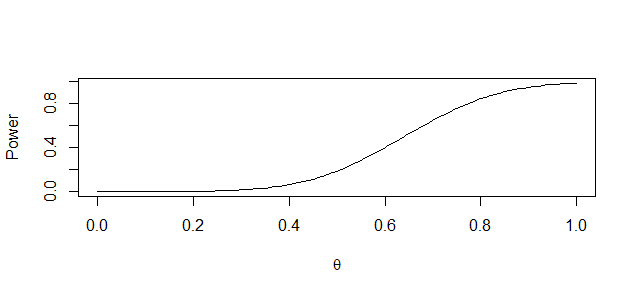
\includegraphics[scale=.8]{Rcode/righttailpower.png}
\pagebreak
	\item 
\begin{multline*}\\
f(y|1/2)=\dfrac{10!}{(10-y)!y!}(1/2)^{10}\\
(1/2)^{10}=\dfrac{1}{1024}\\
\alpha_i=P(Y\leq i|p=1/2) \quad 0\leq i\leq 10\\
\alpha_i=\dfrac{1}{1024}\sum_{y=0}^{i}\dfrac{10!}{(10-y)!y!}\\
{\dfrac{\alpha_y}{1024}}= 1,  10,  45, 120, 210, 252, 210, 120,  45,  10, 1\\
\dfrac{\alpha_i}{1024}=1, 11, 56, 176, 386, 638, 848, 968, 1013, 1023, 1024\\
\alpha_i=\left(\dfrac{1}{1024},\dfrac{11}{1024}, \dfrac{56}{1024},\dfrac{176}{1024},\dfrac{386}{1024},\dfrac{638}{1024},\dfrac{848}{1024},\dfrac{968}{1024},\dfrac{1013}{1024}, \dfrac{1023}{1024},1\right)
\text{ also } \alpha \text{ could equal } 0\\
\end{multline*}
	
\end{enumerate}

	\section*{Problem 3}
	
\begin{enumerate}[(a)]
	\item 
\begin{multline*}\\
f(x|\ta)=\dfrac{e^{x-\ta}}{(1+e^{x-\ta})^2} \quad -\infty <x<\infty, \ -\infty <\ta<\infty\\
\text{For } \ta_2>\ta_1\\
\dfrac{f(x|\ta_2)}{f(x|\ta_1)}=\dfrac{e^{x-\ta_2}}{(1+e^{x-\ta_2})^2}\dfrac{(1+e^{x-\ta_1})^2}{e^{x-\ta_1}}\\
=e^{\ta_1-\ta_2}\left(\dfrac{1+e^{x-\ta_1}}{1+e^{x-\ta_2}}\right)^2\\
T(X)=\dfrac{1+e^{x-\ta_1}}{1+e^{x-\ta_2}}\\
\dfrac{f(x|\ta_2)}{f(x|\ta_1)}=(e^{\ta_1-\ta_2})[T(X)]^2\\
\dfrac{d}{dx}T(X)=\dfrac{e^{x-\ta_1}-e^{x-\ta_2}}{(1+e^{x-\ta_2})^2}\\
\text{because } \ta_2>\ta_1, \ e^{x-\ta_1}>e^{x-\ta_2} \text{ thus the numerator is positive,}\\
\text{making the derivative positive. Thus } T(X) \text{ is increasing.}\\
\text{Since the likelihood ratio depends only on x through } T(X) \text{ and}\\
\text{is a monotone increasing function of } T(X), \text{ the family has MLR}\\ 
\end{multline*}
	
	\item 
\begin{multline*}\\
H_0: \ta=0 \text{ vs } H_1: \ta=1 \quad \alpha=.2\\
\text{Using (N-P) lemmma, the rejection region for the UMP level } \alpha \text{ test is:}\\
R=\{x:f(x|1)/f(x|0)>c \}\\
\text{based on results from part a, this ratio is increasing in x and thus equivalent to:}\\
R^*=\{x:x>c^* \}\\
\alpha=.2=P(x> c^*|\ta=0)\\
(-1)f(x|\ta)\sim Logistic(\ta,-1) \text{ thus:}\\
F(x|\ta)=\dfrac{1}{1+e^{-x+\ta}}\\
.2=1-F(c^*|\ta=0)\Rightarrow.2=1-\dfrac{1}{1+e^{-c^*}}\\
.2=\dfrac{e^{-c^*}}{1+e^{-c^*}}\Rightarrow
.2+.2e^{-c^*}=e^{-c^*}\Rightarrow.2=.8e^{-c^*}\Rightarrow.25=e^{-c^*}\\
c^*=-\log(.25)\approx 1.386\\
\B=P(x\leq c^*|\ta=1)\\
\B=F(c^*|\ta=1)\\
\B=\dfrac{1}{1+e^{-c^*+1}}\Rightarrow \dfrac{1}{1+e^{\log(.25)+1}}\approx 0.5954\\
\B=.5954\\
\end{multline*}

	\item 
\begin{multline*}\\
H_0:\ta \leq \ta_0 \text{ vs } H_1:\ta > \ta_0\\
\text{Since from part a, we have the MLR property holds and }\\
T(x) \text{ is a sufficient statistic then by K-R thm, it is a UMP level } \alpha \text{ test}\\
\text{This is true in general for the logistic location family}\\
\end{multline*}
	
\end{enumerate}
\pagebreak
	\section*{Problem 4}
	
\begin{enumerate}[(a)]
	
	\item 	
\begin{multline*}\\
\samp Pois(\lm)\\
\hyp{\lm\leq \lm_0}{\lm > \lm_0}\\
f(x|\lm)=\pois{\lm}{x} \quad x=0,1,\dots, \ 0\leq \lm <\infty\\
T(X)=\sumx \text{ is a sufficient statistic}\\
T(X)=\sumx\sim Pois(n\lm) \text{ the MLR property holds for } T(X)\\
\text{By K-R thm, the UMP level alpha test is:}\\
R=\{x:\sumx>c \}\\
\alpha=P(\sumn X_i>c|\lm=\lm_0)\\
\end{multline*}

	\item 
\begin{multline*}\\
\hyp{\lm \leq 1}{\lm>1}\\
R=\{x:\sumx>c \}\\
Z=\dfrac{\sumn X_i-n\lm}{\sqrt{n\lm}}\sim N(0,1)\\
\al=.05=P(\sumn X_i>c|\lm=1)\\
.05=P(Z>(c-n)/\sqrt{n})\\
qnorm(1-.05)\approx 1.645\\
\dfrac{c-n}{\sqrt{n}}=1.645\\
c=1.645\sqrt{n}+n\\
\al=.9=P(\sumn X_i>c|\lm=2)\\
.9=P(Z>(c-2n)/\sqrt{2n})\\
qnorm(1-.9)\approx -1.28\\
\dfrac{c-2n}{\sqrt{2n}}=-1.28\\
\text{Plugging in c from the first equation:}\\
\dfrac{1.645\sqrt{n}+n-2n}{\sqrt{2n}}=-1.28\Rightarrow
1.645\sqrt{n}-n=-1.28\sqrt{2n}\\
n=1.645\sqrt{n}+1.28\sqrt{2}\sqrt{n}\Rightarrow
\sqrt{n}=1.645+1.28\sqrt{2}\Rightarrow
n=(1.645+1.28\sqrt{2})^2\\
n=11.93836\approx 12\\
\text{Plugging } n=12 \text{ into the first equation:}\\
(c-12)/\sqrt{12}=1.645\Rightarrow
c=1.645*\sqrt{12}+12\\
c=17.69845\approx 17.7\\
\text{Thus } n=12, \ c=17.7\\
\end{multline*}

\end{enumerate}

	\section*{Problem 5}
	
\begin{multline*}\\
\samp \dfrac{1}{\ta} \quad 0<x<\ta\\
\B(\ta)=P(\xn \leq 1/2 \text{ or } \xn >1|\ta) \quad\ta\in \Theta\\
H_0: \ta=1 \text{ vs } H_1: \ta\neq 1\\
\textbf{Four Cases: } \ta=1 \quad \ta>1 \quad   0<\ta<1/2 \quad 1/2<\ta<1\\
\textbf{Case 1: } \ta=1\\
\B(1)=P(\xn \leq 1/2 \text{ or } \xn >1|\ta=1)\\
=P(\xn \leq 1/2|\ta=1)+P(\xn >1|\ta=1)\\
F_{\xn}(x)=P(\xn\leq x)=\{P(X_1\leq x) \}^n
=\left(\dfrac{x}{\ta}\right)^n=\dfrac{x^n}{\ta^n}\\
P(\xn \leq 1/2|\ta=1)=\dfrac{(1/2)^n}{1^n}=2^{-n}\\
P(\xn >1|\ta=1)=0\\
\B(1)=2^{-n}+0=2^{-n}\\
\B(\ta)=P(\xn \leq 1/2|\ta)+P(\xn >1|\ta)\\
\textbf{Case 2: } \ta>1\\
\B(\ta)=\dfrac{(1/2)^n}{\ta^n}+1-P(\xn\leq 1|\ta)\\
=\dfrac{2^{-n}}{\ta^n}+1-\dfrac{1}{\ta^n}=\dfrac{2^{-n}-1}{\ta^n}+1 \text{ (increasing function of } \ta)\\
\ta\to\infty \quad \pow \to 1 \text{ since:}\\
\dfrac{(1/2)^n-1}{\ta^n}\to 0\\
\textbf{Case 3: } 0<\ta<1/2\\
\B(\ta)=P(\xn \leq 1/2|0<\ta<1/2)+P(\xn >1|0<\ta<1/2)\\
P(\xn \leq 1/2|0<\ta<1/2)=\int_{0}^{\ta}f_{\xn}(x)\dx=\dfrac{x^n}{\ta^n}=\dfrac{1^n}{1^n}=1\\
P(\xn >1|0<\ta<1/2)=0\\
\pow=1+0=1\\
\textbf{Case 4: } 1/2<\ta<1\\
\B(\ta)=P(\xn \leq 1/2|1/2<\ta<1)+P(\xn >1|1/2<\ta<1)\\
\int_{0}^{1/2}f_{\xn}(x)\dx=\dfrac{(1/2)^n}{\ta^n}=\dfrac{2^{-n}}{\ta^n} \text{ (decreasing function of } \ta) \text{ since:}\\
\ta\to\infty \quad \dfrac{2^{-n}}{\ta^n}\to 0\\
\end{multline*}

\end{flushleft}
\end{document}
